\section{Frontend}

Celý frontend naší aplikace je postavený ve Vue.js, moderním
JavaScriptovém frameworku určeného k tvorbě uživatelského rozhraní.
Zaměřuje se na deklarativní renderování a složení komponent.
Pro komunikaci frontendu s backendem pracujeme s REST API, který
pro přenos dat využívá základních protokolů a technologií, jako je
protokol HTTP, přičemž těla požadavků a odpovědí jsou ve formátu JSON.

\subsection{Design UI}

Vzhled uživatelského rozhraní je samozřejmě jednou z nejdůležitějších
vlastností stránky sociální sítě. Lišit se může v závislosti například
na cílové skupině uživatelů, či zaměření sítě. Nicméně, ty nejdůležitější 
obecné principy jsme museli dodržovat a brát v úvahu i při našem návrhu.
Design musí být konsistentní, přehledný a jednoduchý. Když se se stránkou
uživatel setká poprvé, nemusí ho nijak zvlášť ohromit, stačí, aby se v ní
byl hned schopný zorientovat a bezmyšlenkovitě s ní interagovat. Hlavní
funkce a navigace by měly být intuitivní, viditelné a snadno dostupné. 

Je nesmírně důležité, aby byl v celé aplikaci zachován jednotný design 
daných prvků designu (jako jsou např. tlačítka, ikony, či formulářové pole)
a aby si tyto prvky se sebou navzájem dobře vizuálně vycházeli. Proto jsme
v průběhu projektu vybírali jen z úzkého výběru barev, kterými jsou hlavně 
odstíny tmavší šedi, které se navzájem doplňujou, nikoli dráždí. Tyto šedé
tóny konstrastuje pestrá fialová, kterou využíváme k zbarvení a odlišení 
některých funkcí stránky. Křiklavý rozpor šedého pozadí a fialových
detailů uživateli poukazuje na důležitost těchto funkcí. Touto fialovou se
rozhodně šetří, zesiluje tím právě dojem její rarity a důsledně i hodnoty.
Právě touto barvou se hlavně chlubí všudypřítomné tlačítko "New Post" 
(Nový příspěvek), které i svou velikostí je pro uživatelé naproto
nepřehlédnutelné.

Vedle barev prkvů je ale samozřejmě důležitý i jejich tvar a viditelný obsah.
Chtěli jsme, aby stránka působila přátelsky a přívětivě. Všechna tlačítka,
příspěvky a inputové pole jsou zaoblovány, zdají se tak sympatičtější. Na 
ostrou hranu prakticky napříč celým programem nenarazíte, tento trend ctí
i font hlavního loga, se kterým se nový uživatel setkává například hned u
vytváření vlastního účtu. I ikony ze sady "heroicons", se kterými jsme se
rozhodli pracovat, na oko působí příjemně.

\begin{figure}[h!] 
    \centering
    
\includegraphics[width=0.6\textwidth]{images/dinglogo.png}
    \caption{Logo Ding}
    \label{ding-logo}
\end{figure}

\subsection{Router}

Vue router je oficiální router pro Vue.js. Důvodem, proč jsme se rozhodli
pracovat s Vue router je, že nám umožňuje přepínat mezi jednotlivými stránkami
bez nutnosti načítat celou stránku znovu, což je výhodné pro uživatele, protože
se mu stránka bude načítat rychleji, což zlepší celkový dojem z aplikace.
% ...

\subsection{Komponenty}

Komponenty jsou základní stavební jednotkou Vue.js aplikace. Využíváme je
k vytvoření uživatelského rozhraní. Komponenty jsou znovupoužitelné a díky tomu
nemusíme po každé vytvářet stejné bloky kódu, tudíž šetříme čas a zjednodušujeme
si práci. Importujeme je do souboru, kde je můžeme zavolat. Komponenty jsou velmi
užitečné pro vytváření opakujících se elementů, jako jsou například příspěvky, 
komentáře, nebo nastavení uživatelského profilu. 

\subsection{Vytváření nového příspěvku}

Uživatel může nový příspěvek vytvořit po kliknutí na tlačítko "New Post" na domovské
stránce. Po kliknutí na tlkačítko je uživatel přesměrován na stránku, kde může
vytvořit nový příspěvek. Uživatel může příspěvek vytvořit dvěma způsoby, buť nahráním 
audio souboru ze zařízení, nebo nahráním zvuku pomocí mikrofonu. Pokud uživatel 
začne nahrávat zvuk pomocí mikrofonu, tak se mu zobrazí vizualizér. vizualizér se
mu zobrazí i v případě, že nahrává audio soubor ze zařízenní a začne ho přehrávat.

\subsubsection{Vizualizér}

Vizualizér se uživateli zobrazí ve chvíli, co začne pomocí mikrofonu nahrávat zvuk,
či po zahájení přehrávaní nahraného audio souboru. Je vytvořený pomocí "web audio API"
a HTML elementu \texttt{<canvas>}. Na canvas se vykresluje linka, která mění svou výšku podle
hlasitosti zvuku. Ta je získána pomocí \texttt{AnalyserNode}. Délka linky je omezená, aby
se nezobrazovala mimo canvas. Tohoto jsme docílili pomocí \texttt{Queue} datové struktury, 
která jak název napovídá je fronta. Jakmile se linka dostane na konec canvasu, tak se 
vykreslovat nepřestane, akorát se zleva postupně stará data odebírají.

AnalyserNode přijímá zvukový signál a generuje výstupní data, která obsahují
informace o frekvenčním spektru a hlasitosti signálu. Tyto informace používáme 
k vizualizaci zvukového signálu skrze metodu \texttt{getByteFrequencyData()}, která
umožňuje získávání informací o frekvenčním spektru signálu v podobě pole bytů,
kde každý prvek pole reprezentuje hlasitost signálu v daném frekvenčním pásmu. \autocite{analysernode-mdn}

AnalyserNode má také několik vlastností, které ovlivňují jeho chování.
Vlastnost \texttt{fftSize} určuje množství frekvencí, které FFT (Fast Fourier Transform) algoritmus
rozeznává.

\begin{figure}[h!] 
    \centering
    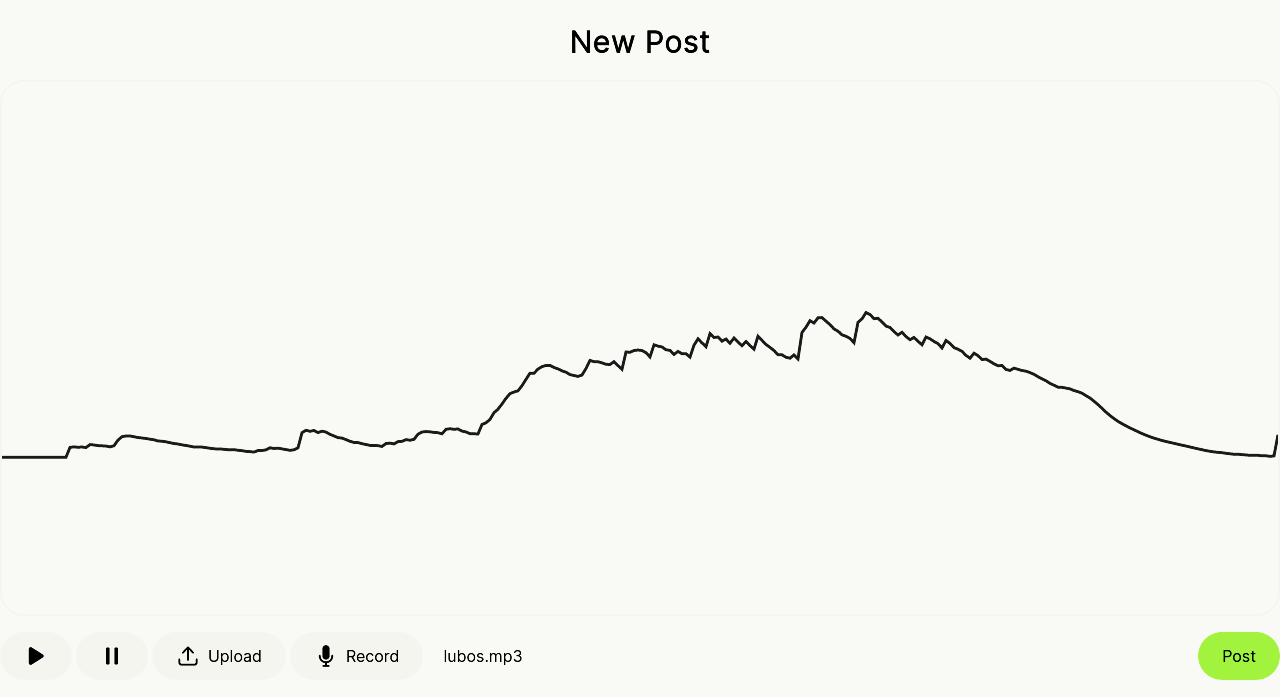
\includegraphics[width=0.7\textwidth]{images/vizualizer.png}
    \caption{Vizualizér}
    \label{vizualizer}
\end{figure}
